\section{Deep CFR: the ledger becomes a regression problem}\label{sec:deepcfr}

\mkey{deep cfr}Now the pieces assemble into the project's centerpiece. At full Drawmaha scale no table fits, and \keyterm{Deep CFR}\mdef{Deep CFR}{CFR where neural networks predict the regret ledger's contents instead of storing them} (Brown, Lerer, Gross \& Sandholm 2019~\cite{brown2019deep}) makes the one substitution left to make: everything about CFR stays --- external-sampling traversals, regret matching, average-vs-current --- but the per-infoset ledger is replaced by a network trained to \emph{predict} what the ledger would contain, generalizing across the millions of hands that were never sampled. The bet is statistical: similar hands should regret alike, so every sample teaches a neighborhood, and bucketing is learned end-to-end instead of hand-engineered. It was the first non-tabular CFR to work in large poker, beating NFSP on exploitability (37 vs.\ 47 mbb/hand on Flop Hold'em) and playing competitively against a $3.3\times10^8$-bucket abstraction in full limit hold'em.

\begin{figure}[t]
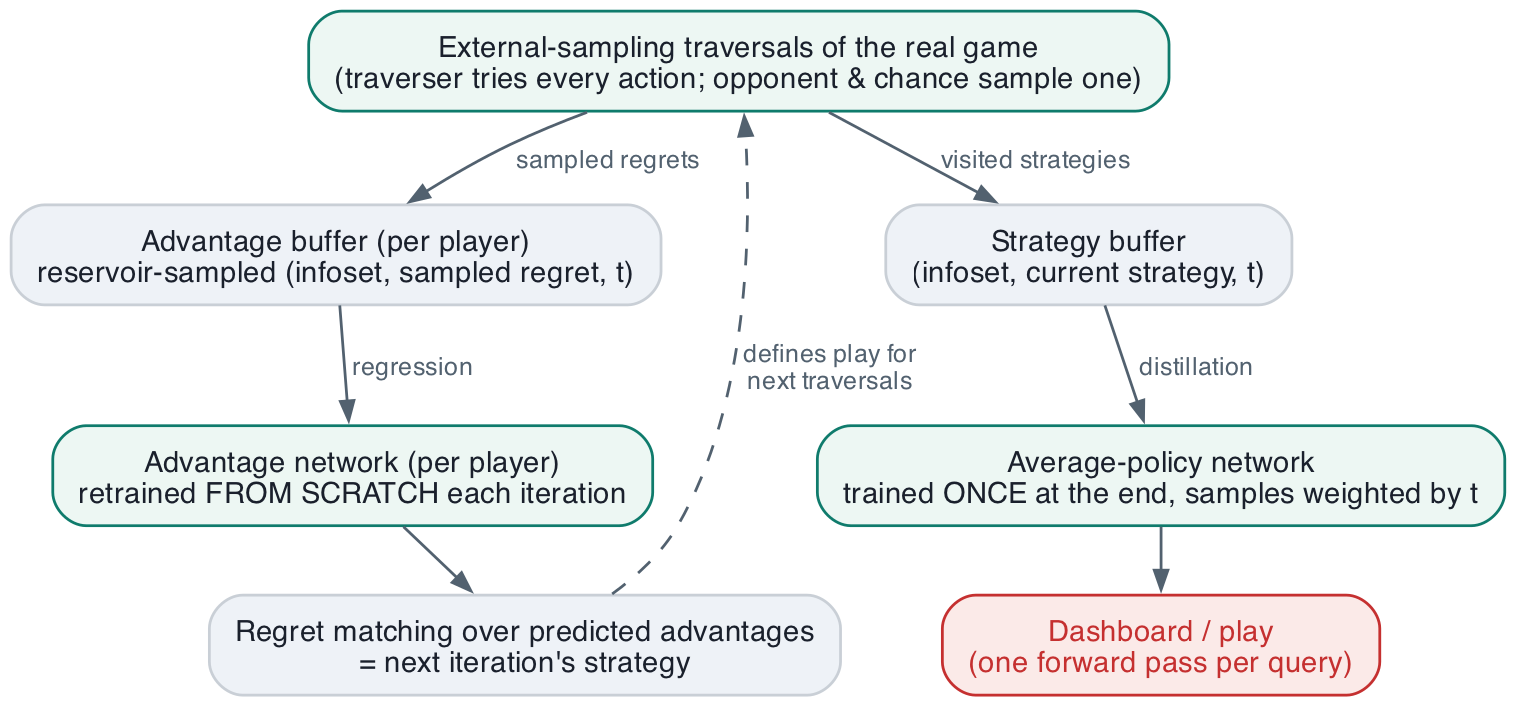
\includegraphics[width=\linewidth]{figures/pipeline.png}
\caption{The Deep CFR training loop; teal = learned components, red = what the dashboard queries.}
\label{fig:pipeline}
\end{figure}

Walking Figure~\ref{fig:pipeline} clockwise:
\begin{enumerate}
\item \textbf{Traverse.} Run external-sampling traversals of the \emph{real} game (Section~\ref{sec:mccfr}); the current strategy at any infoset is regret matching over the advantage network's predictions.
\item \textbf{Collect.} Each traversal writes (infoset features, sampled instantaneous regret, iteration $t$) tuples --- \keyterm{advantages}\mdef{advantage (CFR sense)}{a sampled instantaneous counterfactual regret; the regression target, NOT actor--critic's advantage} --- into a per-player buffer, and (infoset, current strategy, $t$) into a strategy buffer.
\item \textbf{Regress.} Each iteration trains that player's advantage network \emph{from scratch} on its buffer. From scratch is not paranoia: cumulative regrets are nonstationary, and the paper's ablation shows fine-tuning one network across iterations converges substantially worse.
\item \textbf{Average.} At the very end, one \keyterm{average-policy network}\mdef{average-policy network}{a net distilled from all iterations' strategies, weighted by $t$ --- the deployable equilibrium approximation} is distilled from the strategy buffer with samples weighted by $t$ (Linear-CFR weighting, Section~\ref{sec:speedups}). \hlight{That single network IS the solver output --- the thing the folk theorem blesses, the thing the dashboard queries at one forward pass per hand.}
\end{enumerate}

\begin{intuition}{reservoir buffers: a fair fixed-size memory of an endless stream}
The buffers cannot hold every sample ever generated, and a FIFO buffer would remember only recent iterations --- but the \emph{average} strategy needs all of history represented fairly. Reservoir sampling keeps a fixed-size buffer that is, at every moment, a uniform random sample of everything seen so far: each new item displaces a random resident with exactly the right probability. Deep CFR's guarantees lean on this fairness; swapping in a FIFO buffer is a known way to quietly break convergence.
\end{intuition}

\begin{lstlisting}
for t in 1..T:                                # Deep CFR outer loop
  for p in players:
    for k in 1..K:                            # e.g. K = 10,000 traversals
      traverse(deal(), p, adv_net[p], adv_buf[p], strat_buf, t)
    adv_net[p] = train_from_scratch(adv_buf[p],   # regression on
                   target="sampled regret", weight="t")  # ledger contents
final = train(strat_buf, target="strategy", weight="t")  # average-policy net
# play/dashboard: sigma(I) = regret_match(final(I))  -- one forward pass
\end{lstlisting}

\subsection*{The published recipe, as starting hyperparameters}

Deep CFR's appendix is a de-risked starting point, small enough to be encouraging:

\begin{center}
\footnotesize
\begin{tabular}{@{}ll@{}}
\toprule
Network & 7 layers, $\sim$99K parameters: card branch + bet branch \\
Card encoding & rank + suit + card embeddings, summed within permutation-invariant groups \\
Bet encoding & per betting slot: occurred-flag + bet size as pot fraction \\
Buffers & 40M samples each (advantage $\times2$, strategy), reservoir-sampled \\
Per iteration & 10K traversals; retrain 4K SGD steps, batch 10K \\
Optimizer & Adam, lr $10^{-3}$, gradient-norm clip 1 \\
Small-game anchor & (SD-CFR, Leduc): $3\times64$ nets, 1M buffers, 1.5K traversals/iter \\
\bottomrule
\end{tabular}
\end{center}

The card-embedding scheme transfers to Drawmaha almost verbatim --- permutation invariance over hole cards only grows in value with 5-card hands --- but two encoding questions have \emph{no} published answer and are flagged now as genuine design work: how the 32-subset \textbf{discard action} should be headed (flat 32-way output vs.\ per-card keep/discard logits --- regret matching over a factorized action space is unexplored territory), and how both players' public \textbf{draw-count histories} (plus the face-up draw-1 card) enter the input features. Section~\ref{sec:checklist} carries both.

\subsection*{The forks in the neural-CFR family}

\mkey{sd-cfr / dream / escher}Successors map the design space, and three matter here. \textbf{SD-CFR} (Steinberger 2019~\cite{steinberger2019}) deletes the average-policy network: since the average strategy is just an iteration-weighted mixture of per-iteration strategies, and each is recoverable from that iteration's advantage net, storing every checkpoint ($\sim$400KB each) reconstructs the \emph{exact} average --- one less approximation, measurably better exploitability. Its cost is inference: querying means evaluating many checkpoints, awkward for a live dashboard. \mnote{Best of both, and the plan: train SD-CFR-style (keep checkpoints, evaluate exactly), distill ONE average-policy net at the very end for serving.}\textbf{DREAM} (2020~\cite{steinberger2020dream}) and \textbf{ESCHER} (2022~\cite{mcaleer2022}) exist for simulator-free settings: outcome sampling forces importance weights, whose variance takes an extra learned baseline network (DREAM) or a learned history-value function under a fixed sampling policy (ESCHER) to control. Their lesson for a project that \emph{owns} its simulator is purely diagnostic: \hlight{importance-sampling variance is what kills neural CFR at scale --- choose external sampling on day one and the whole problem never appears.}

Two pitfalls close the section, both documented failure modes. \pitfall{Forgetting the iteration-$t$ weighting on strategy-buffer samples silently converges to the wrong average} --- a classic bug, since nothing crashes. And the loss curves of advantage networks are \emph{expected} to look bad: cumulative regrets grow and drift across iterations (the nonstationarity ReCFR~\cite{liu2022recfr} formalizes), so a plateauing or climbing regression loss is often target drift, not optimizer failure --- one more reason Section~\ref{sec:evaluation} insists exploitability curves, never training losses, are the progress signal.
